%%
%% This is file `thesis.tex',
%% generated with the docstrip utility.
%%
%% The original source files were:
%%
%% nudtpaper.dtx  (with options: `thesis')
%%
%% This is a generated file.
%%
%% Copyright (C) 2013 by Liu Benyuan <liubenyuan@gmail.com>
%%
%% This file may be distributed and/or modified under the
%% conditions of the LaTeX Project Public License, either version 1.3a
%% of this license or (at your option) any later version.
%% The latest version of this license is in:
%%
%% http://www.latex-project.org/lppl.txt
%%
%% and version 1.3a or later is part of all distributions of LaTeX
%% version 2004/10/01 or later.
%%
%% To produce the documentation run the original source files ending with `.dtx'
%% through LaTeX.
%%
%% Any Suggestions : LiuBenYuan <liubenyuan@gmail.com>
%% Thanks Xue Ruini <xueruini@gmail.com> for the thuthesis class!
%% Thanks sofoot for the original NUDT paper class!
%%
%1. 规范硕士导言
% \documentclass[master,ttf]{nudtpaper}
%2. 规范博士导言
% \documentclass[doctor,twoside,ttf]{nudtpaper}
%3. 如果使用是Vista
% \documentclass[master,ttf,vista]{nudtpaper}
%4. 建议使用OTF字体获得较好的页面显示效果
%   OTF字体从网上获得,各个系统名称统一,不用加vista选项
%   如果你下载的是最新的(1201)OTF英文字体,建议修改nudtpaper.cls,使用
%   Times New Roman PS Std
% \documentclass[doctor,twoside,otf]{nudtpaper}
%   另外,新版的论文模板提供了方正字体选项FZ,效果也不错哦
% \documentclass[doctor,twoside,fz]{nudtpaper}
%5. 如果想生成盲评,传递anon即可,仍需修改个人成果部分
% \documentclass[master,otf,anon]{nudtpaper}
%
\documentclass[doctor,twoside,otf]{nudtpaper}
\usepackage{mynudt}

\classification{TP393}
\serialno{14069001}
\confidentiality{公开}
\UDC{}
\title{GPU}
\displaytitle{GPU}
\author{李晨}
\zhdate{\zhtoday}
\entitle{Research on GPU}
\enauthor{Li Chen}
\endate{\entoday}
\subject{电子科学与技术}
\ensubject{Electronic Science and Technology}
\researchfield{信息安全技术}
\supervisor{郭阳\quad{}研究员}
\cosupervisor{} % 没有就空着
\ensupervisor{Researcher Guo Yang}
\encosupervisor{}
\papertype{工学}
\enpapertype{Engineering}
% 加入makenomenclature命令可用nomencl制作符号列表。

\begin{document}
\graphicspath{{figures/}}
% 制作封面,生成目录,插入摘要,插入符号列表 \\
% 默认符号列表使用denotation.tex,如果要使用nomencl \\
% 需要注释掉denotation,并取消下面两个命令的注释。 \\
% cleardoublepage% \\
% printnomenclature% \\
\maketitle
\frontmatter
\tableofcontents
\listoftables
\listoffigures

\midmatter
\begin{cabstract}
为了延缓摩尔定律的终结,人们开始从半导体技术以外的方向来提升芯片的性能。
在这些新方向中,堆叠技术和异构众核加速技术已经逐渐被认可,并得到了广泛的应用。
堆叠异构系统如今已成为数据中心重要的硬件基础,随着云计算的不断发展和广泛应用,堆叠异构系统开始为云计算提供强大的计算加速能力。

然而,云计算的软硬件资源以服务的形式同时提供给大量租户,而多租户之间完全隔离。
用户难以从纯软件角度在云环境中针对硬件特征进行性能优化。
因此,应用透明的性能优化策略显得尤为重要。

本文针对堆叠异构系统中的内存超额配置造成的性能骤降问题、多任务抢占的上下文切换高开销问题和堆叠互连网络结构的负载不均衡问题,
提出了一系列应用透明的策略,在不修改应用程序代码的前提下,高效地优化应用程序的性能。
本文的主要研究成果及创新点如下:

(1)提出了一种内存超额配置管理框架

如今云服务提供商往往将超出其硬件资源的服务提供给用户,以提高资源利用率。
但是,对于一些对资源需求较高的用户(如深度学习训练),很容易出现内存紧缺的问题。
当代GPU已经能够支持内存超额配置,但是我们实验发现在内存超额配置的情况下,应用程序遭受了严重的性能损失,亟需一种应用透明策略来应对。
本文研究了多种应用程序的访存特性,为不同的内存超额配置开销提出了主动数据页逐出技术、内存感知的并行度管理策略和内存容量压缩策略。
本文提出了一种内存超额配置管理框架,在线判断应用程序的类别,并选择相应的策略组合来实现内存超额配置下的性能提升。
实验表明,本文的内存超额配置管理框架能够大幅度恢复由于内存超额配置导致的性能损失。

(2)提出了一种动态采用检查点备份技术的GPU主动抢占策略

多任务处理机制已经在堆叠异构系统中广泛应用,
而抢占机制则是多任务处理中必不可少的一环。
抢占机制能够满足不同应用程序对于服务质量的要求,同时也为多任务切换提供了更多选择。
然而,GPU由于其单指令多线程的特性,其上下文大小相比于CPU的上下文大小显著增加,上下文切换开销也相应增大。
本文为解决这一问题,观察了GPU内核函数的启动过程,动态采用检查点备份的主动抢占机制来降低上下文切换的开销。
实验表明,本文的主动抢占机制可以将抢占延迟从平均8.9$\mu$s降低到平均3.6$\mu$s,应用程序也因此更容易满足服务质量的要求。

(3)提出了一种动态延迟感知的2.5维堆叠片上网络负载均衡策略

2.5维堆叠片上网络是一种面向硅中介层堆叠的新型结构,利用硅中介层上的大量连线资源,新增加一层网络结构分担网络流量。
但是,当前的设计将上层网络用于计算核心节点之间的协议通信,而下层网络用于访存通信。
我们对于PARSEC测试集的测试发现,上下层网络会出现严重的负载不均衡现象,并且路径拥塞情况有助于判断网络拥塞与否。
因此,本文提出了一种延迟感知的2.5维堆叠片上网络负载均衡策略,通过延迟感知来判断拥塞路径,并为报文的路径做出路由选择。
实验表明,本文提出的负载均衡策略相比于基准方法有45\%的性能提升。

综上所述,本文面向堆叠异构系统,紧紧围绕``应用透明''的需求,
针对内存超额配置、多任务切换管理和网络负载不均衡问题,研究了产生应用程序性能损失的原因、应用程序的特征和硬件特性,
分别提出了有效解决方案,并都取得了系统性能的提升。
因此,本文的成果在理论上可以为软硬件设计提供了指导,同时具有重要的工程价值。

\end{cabstract}
\ckeywords{堆叠技术;异构系统;应用透明;内存超额配置;虚拟内存;多任务切换;片上网络;负载均衡}

\begin{eabstract}
In order to delay the ending of Moore's law, more emerging techniques appear to improve the chip performance in new ways, rather than traditional semiconductor methods.
In these new directions, stacking technology and heterogeneous many-core acceleration technology have been gaining more tractions and they are widely used in commercial products.
Stacked heterogeneous systems become important hardware resources in data centers. 
With the advancement and widespread application of cloud computing, stacked heterogeneous systems start providing powerful abilities of computing acceleration for cloud computing.

However, the hardware and software resources of cloud computing are provided to a lot of users as services.
Due to the complete isolation among multi-tenancy, it is difficult for programmers to perform application optimization in cloud environments from software perspective.
Therefore, it is important to apply application-transparent performance optimization strategies based on hardware features.

This thesis addresses three issues, including the performance degradation caused by memory oversubscription in a heterogeneous system, the high overhead of context-switching in multi-tasking preemption, and the load imbalance of the stacked interconnect network.
Several application-transparent strategies are proposed to solve these issues and efficiently optimize the performance without modifying the applications' code.
The main contributions and innovations of this paper are shown as follows:

(1) a framework for memory oversubscription management

Nowadays, cloud providers usually virtualizes costly hardware resources for users to increase the resource utilization.
However, it may cause the memory shortage for some memory-hungry users (such as machine learning training).
Memory oversubscription has been enabled in modern GPUs.
However, our measurements on a real GPUs shows that memory oversubscription can casue severe performance degradation.
An application-transparent mechanism is urgently needed.
In this thesis, we investigate the memory access behaviors of different applications, 
and we propose proactive eviction, memory-aware throttling and capacity compression to address different overheads.
Our framework for memory oversubscription management is proposed to select the most effective combination of these techniques to recover the performance loss caused by memory oversubscription according to the application type. 
Experimental results show that our framework is effective at improving the performance under the memory oversubscription. 

(2) a dynamic and proactive preemption preemption mechnism using checkpointing

Multi-tasking has been widely used in stacked heterogeneous systems.
The preemption support is a necessary technique for multitasking.
The preemption can satisfy the quality of service requirements of different applications, and it provides more options for multi-tasking switching as well.
However, due to its SIMT model, the GPU has much larger context size compared with CPU, and the overhead of context switching is also increasing.
In order to address this issue, we observe the launching process of GPU kernels, and dynamically adopts the proactive preemption mechanism using checkpointing to reduce the overhead of context switching.
Experimental results show that our proactive preemption mechanism can reduce the latency from 8.9$\mu$s to 3.6$\mu$s, making it easier to meet quality of service requirements.

(3) a dynamic latency-aware load-balancing strategy in 2.5D NoC architecture

The 2.5D stacking on-chip network is an emerging structure for silicon interposer architecture. 
It utilizes the abundant metal resources on the silicon interposer to create a new layer of network.
As a result, it can hold those congested network traffic.
However, in current design, the protocol-level traffic among cores is transfered on upper level network, while the memory traffic is transfered on the lower layer.
Our measurements on the PARSEC benchmark show that there is a severe load imbalance between the upper and lower layers.
We find that the accurate network congested information can be observed from the congested path. 
Therefore, this thesis proposes a latency-aware load balancing strategy in 2.5D NoC architecture.
The congestion path is determined by the latency, and the path selection of packets is made.
Experimental results show that our load balancing strategy has a 45\% performance improvement over the baseline.

In summary, this thesis focuses on the stacking heterogeneous system. 
It aims the need for ``application transparency''.
For issues of memory oversubscription, multi-tasking switching management and network load imbalance, the reason of these performance losses, application characteristics and hardware features are studied.
Finally, we propose effective solutions to address these issues and the system performance are improved.
Therefore, this thesis has both engineering value and theoretical significance.

\end{eabstract}
\ekeywords{Stacking Technology, Heterogeneous System, Application-transparent, Memory Oversubscription, Virtual Memory, Multi-task Switch, Network-on-Chips, Load-balancing}


%\input{data/denotation}

%书写正文,可以根据需要增添章节; 正文还包括致谢,参考文献与成果
\mainmatter
\chapter{绪论}
\label{chap:intro}
近几十年来,随着半导体技术的不断发展,计算机系统的性能成几何级增长。
一方面,由于半导体工艺的不断进步,晶体管尺寸不断缩小,芯片能够集成的晶体管数目不断增大;
另一方面,也是因为硬件系统结构、编译技术和算法的不断发展和进步。
在这些性能增长中,晶体管尺寸的缩减起到了决定性作用~\upcite{hennessy2011computer}。
然而,从2005年开始,量子隧穿效应使得晶体管漏电现象开始出现。
晶体管尺寸由于受到小晶体管静态功耗的影响,已经难以再按照登纳德缩放比例定律(Dennard Scaling)~\upcite{dennard1974design}继续缩减,
时钟频率难以继续提升。
为了继续提升性能,就必须从更高效的体系结构上下功夫。多核处理器、配有专用硬件加速器的异构系统应运而生。

研究发现,专用硬件加速器能够显著提升处理器的能效比~\upcite{hameed2010understanding}。 
无论是传统的DSP~\upcite{chen2014ft}、GPU~\upcite{volta, pascal, fermi, amd-fusion, radeon},还是针对深度神经网络加速的谷歌TPU~\upcite{Jouppi:2017:IPA:3079856.3080246}、寒武纪AI加速器~\upcite{chen2014diannao,chen2014dadiannao},这些加速器与CPU组成异构系统。
该体系结构通过将大量并行计算或专用计算任务从CPU发送到GPU、DSP或其他专用加速器,显著减少了CPU指令执行的开销和程序员的负担,系统性能和能效均显著提高,
对于图像处理、高性能计算、以及深度学习训练~\upcite{krizhevsky2012imagenet,simonyan2014very,szegedy2015going,zeiler2014visualizing}都具有重要作用。
在这之中,GPU处理器的应用最为广泛,据Hameed等人的研究表明,一个GPU的运算处理性能通常不低于10个CPU核~\upcite{hameed2010understanding}。
虽然起初其出现的主要目标是解决CPU对图像渲染加速不足的问题,但由于其架构在处理并行计算的天然优势,使得GPU目前更多地被用于通用并行计算~\upcite{bolz2003sparse,fan2004gpu,he2008mars}。
如今无论是手机、平板电脑、笔记本,还是数据中心和超级计算机,GPU已无处不在。

异构系统不断发展,应用规模和数据规模不断增长,又遇到了存储墙问题,访存开销越来越大。
在此背景之下,为了继续维持摩尔定律,提升集成电路性能的同时降低集成电路的开销,\texttt{集成电路堆叠技术}~\upcite{Xie:2015:DA:2842825,loh-ieeemicro2007, samsung-pr2007,black2013stacking}成为一种有效解决方案被广泛应用。
三维堆叠集成技术是一种新的集成电路工艺,将多个硅片垂直堆叠并以三维封装的方式封装成一个芯片,
是在工艺尺寸缩减受限的情况下提高系统性能的一种新的方式。
三维堆叠集成电路技术从\texttt{延伸摩尔定律}和\texttt{超越摩尔定律}两方面实现芯片上晶体管密度和芯片性能的大幅度提升,
在提升带宽、降低延迟和提高能效方面有许多优势。不过,受限于良率、热效应、设计复杂度、设计测试成本以及EDA工具等方面的限制,
三维堆叠技术目前主要用于一些如存储器等互连简单、单元排列重复的规则电路。
相比于三维堆叠技术这种革命性的革新,\texttt{基于硅中介层的2.5维堆叠技术}则属于一种进化技术,避免了三维堆叠技术中的各种问题。
2.5维堆叠集成电路是将多个同构或异构的部件相邻地堆叠在硅中介层上,相邻部件之间通过硅中介层进行通信。
通过2.5维堆叠可以将处理器和三维堆叠存储器相邻地堆叠在硅中介层上,为处理器增加内存容量的同时显著提高内存带宽,已经广泛用于目前商业化的异构处理器中。


\section{研究动机}
高性能堆叠异构系统目前已经被引入数据中心,为云计算~\upcite{mell2011nist,dillon2010cloud,hauswald2015sirius}提供更加强大的计算和存储能力。
云计算中\texttt{多租户技术}的应用使得多个用户能够共享高性能堆叠异构处理器,并同时执行和处理多个任务。
无论是\texttt{IaaS}~\upcite{bhardwaj2010cloud}、\texttt{PaaS}~\upcite{vaquero2008break}、还是\texttt{SaaS}~\upcite{koomey2011growth},均对多租户技术有着强烈的需求。
多租户任务允许计算资源的共享和存储资源的相互隔离,同时需要保证多租户任务间的安全隔离性。
虽然多租户技术保证了安全隔离性,但用户无法了解任务运行的具体情况,难以从程序员的角度对应用程序进行优化,
因此,研究面向堆叠异构系统的应用透明策略显得尤为重要。

本文从堆叠异构系统出发,发现并解决堆叠异构系统的三大问题:

\textbf{内存超额配置造成的性能骤降问题。}
云提供商往往会给用户提供超过其硬件资源的存储资源,在用户不同时使用这些资源的情况下提高数据中心的资源利用率。
然而随着用户应用规模和数据量的不断增大,内存超额配置越来越普遍。
堆叠异构处理器,如GPU,目前已经能够为用户提供内存超额配置的支持。
但通过我们在真实GPU的实验发现,当内存超额配置时,GPU出现了严重的性能下降,在一些情况下甚至会发生宕机。

\textbf{多任务抢占的高上下文切换开销问题。}
为在多任务处理中快速响应一些优先级较高,对延迟比较敏感的任务,必须支持多任务抢占机制进行快速切换。
上下文切换是多任务抢占的一种重要方式。
然而GPU等堆叠异构系统相对于CPU,由于其同时处理大量数据,上下文大小相对较大。
因此,GPU上下文切换的开销远大于CPU,传统的上下文切换机制占用的存储带宽将严重影响多任务抢占的性能。

\textbf{堆叠互连网络结构的负载不均衡问题。}
在2.5维堆叠异构系统中,传统的方式是在相邻处理器或存储器的四周边缘通过硅中介层进行互连。
Enright Jerger等人~\upcite{jerger2014noc}提出利用硅中介层大量的连线资源设计了2.5维片上互连网络。
一般情况下,该网络结构通过上层网络进行一致性协议报文的通信,通过下层网络进行访存报文的通信。
但是,我们的实验发现,由于不同类型报文的不均衡性,该方法会导致上下层网络的负载不均衡问题,严重影响整个系统的性能。

本文的研究发现,传统的通过程序员手工调试优化的技术都难以在支持多租户技术数据中心中高效使用。
本文针对堆叠异构系统中的上述三大问题,研究对应用透明的硬件或驱动策略,
使得堆叠异构系统能够在程序员不修改应用程序的前提之下为这些问题提供高效的解决方案。

\section{研究内容和主要贡献}

\subsection{研究内容}
本文面向堆叠异构系统,研究对应用透明、程序员不感知的优化策略,解决上述三大问题,主要包括:

(1)一种内存超额配置管理策略框架(ETC)

现代分立式GPU支持统一内存技术和实时按需取页技术。这种在CPU和GPU内存中自动的数据拷贝管理显著降低了开发者的负担。
但是,当应用程序的在线工作数据集超过GPU物理内存时,产生的额外数据移动会导致严重的性能损失。

本文提出了一种内存超额配置管理框架(ETC),采用了一系列对应用和程序员透明的新技术提升内存超额配置下的GPU性能。
主要思想包括掩藏数据页逐出延迟、降低内存抖动开销、以及增大有效的内存空间。
数据页逐出延迟可以通过\texttt{主动数据页逐出技术}尽早为将要取进来的数据页腾出空间,掩藏延迟;
内存抖动的开销可以通过\texttt{内存感知的并行度控制策略},动态地将GPU的并行度降低以减少在线工作数据集的大小,缓解内存抖动现象;
\texttt{内存容量压缩技术}在不需要增大物理内存容量的前提下使得更大的在线工作数据集能够被内存容纳。
我们发现没有任何一种技术对所有类型的应用程序都有效。因此,我们的ETC将\texttt{主动数据页逐出技术}、\texttt{并行度控制策略}和\texttt{内存容量压缩技术}
集成到一个管理框架,当内存超额配置时针对应用程序类型动态地选择这些策略的组合,对应用程序透明的提升GPU的性能。
从这个角度出发,ETC将应用程序划分为无数据共享的规则应用程序、数据共享的规则应用程序以及不规则的应用程序。

实验分别实现了一种当前的基准结构、一种具有无限内存大小的理想结构以及我们的设计ETC。
ETC几乎能够完全消除无数据共享的规则应用程序的内存超额配置开销,使之性能与具有无限内存空间的理想情况类似。
我们还发现,相比于当前的基准策略,我们的ETC能够将数据共享的规则应用程序和不规则应用程序的内存超额配置开销显著降低。

(2)一种动态采用检查点备份技术的GPU主动抢占策略(PEP)

无论是空间上的多任务支持还是时间上的多任务支持,GPU对多任务处理的需求都在不断增加。
这要求GPU可以随时被高优先级应用程序抢占,在某一应用程序正在执行的过程中,中断执行并切换上下文到新的应用程序。
不同于CPU,GPU由于其大量的上下文大小,上下文切换产生的开销非常大。
研究人员已经做出了大量工作来降低GPU上的抢占开销。
例如降低上下文的大小或将上下文切换和程序执行重叠等。
而所有之前的这些方法都是被动式的,意味着上下文切换都是在抢占请求到来之后才开始的。

本文提出了一种动态主动的抢占机制(PEP)来降低抢占的延迟,我们观察到GPU内核函数的执行无论是在CUDA还是OpenCL下都一定是在内核函数启动后开始的。
因此,抢占请求可以在其实际到达GPU前预测。我们研究了这一段延迟,并开发了一种预测机制提前进行状态备份。
当抢占请求实际到达GPU后,我们只需要将相对于上一次状态备份的增量部分再做备份,非常类似于传统的检查点备份技术。
我们的设计同时也可以根据GPU内核函数在运行过程中的特性动态选择\texttt{排空执行技术}或\texttt{基于检查点的上下文备份技术}。
实验测试结果表明,PEP设计可以有效的降低等待上下文切换产生的停滞延迟。
此外,PEP的脏上下文备份机制也有效地减少了需要备份的上下文的大小。

(3)一种动态延迟感知的2.5维堆叠片上网络负载均衡策略(DLL)

由于三维堆叠技术依然面临许多的挑战,当前2.5维堆叠技术具有更好的应用前景。
通过硅中介层的应用,2.5维堆叠技术可以为异构处理器提供更高带宽和更大容量的存储系统。
为了满足2.5维堆叠芯片的存储系统通信要求,可以硅中介层上丰富的连线资源可以来开发并实现一套新的网络。
但是,实验发现2.5维堆叠片上网络体系结构的性能受到两层网络之间严重的不均衡负载限制,难以发挥出应有的性能。

为了解决这个问题,本文提出了一种动态延迟感知的负载均衡策略(DLL)。
核心想法是通过最近几个报文的平均延迟来检测整个网络层的拥塞程度,
根据收集到的数据在每个源节点进行报文网络层的路由选择。
我们利用了硅中介层上充足的连线资源实现了一个延迟传播环网,
确保在目的节点收集到的报文延迟信息能够传输回源节点,
采用这些信息进行路由选择达到了负载均衡的目标。

实验将DLL策略的实现与无负载均衡策略的基准设计、一种目的节点检测的策略和一种缓存感知的策略的实现进行比较,
我们的DLL策略均达到了吞吐率提升,同时产生的开销非常小。


\subsection{主要贡献}
本文系统深入地研究了应用透明策略以提升堆叠异构系统的性能,取得了许多系统性开创性的成果,主要创新点如下:

(1)提出了一种内存超额配置的管理框架

内存超额配置虽然在当前GPU中得到了完全支持,但之前的工作没有考虑内存超额配置所带来的严重开销,
且内存超额配置的优化工作都需要修改应用程序,难度较大且效果不一定好。
本文提出了一种内存超额配置的管理框架,主要贡献包括:
\renewcommand*\theenumi{(\alph{enumi})}
\begin{enumerate}
\setlength\itemsep{1pt}
\item 据我们所知,这是第一个对GPU内存超额配之下的性能开销做深度分析的工作。
通过对应用程序访存trace的分析,找出了不同应用程序类型在GPU内存超额配置下出现严重性能损失的不同原因。
\item 提出了一种软硬件结合的对应用透明的解决方案,能够显著降低内存超额配之下的性能损失。
该方法对程序员不感知,不需要任何应用程序代码的修改。
\item 开发了三种内存超额配置的优化策略。我们发现并没有任何一种单一方法能够对所有类型的应用程序都见效。
从这个角度出发,本研究的策略根据访存特性,在线划分应用程序的类别,并为不同类别的应用程序采用不同的策略组合进行性能优化。
\end{enumerate}

该部分的研究成果~\upcite{Li:asplos19}发表在系统结构领域的顶级会议第24届ACM国际编程语言与操作系统的体系结构支持会议
(The 24th ACM International Conference on Architectural Support for Programming Languages and Operating Systems, ASPLOS-19)上。

(2)提出了一种动态采用检查点备份技术的GPU主动抢占策略

GPU中的多任务抢占开销非常大,这是由于相对于CPU,GPU的上下文较多,需要备份的上下文数据较大。
传统的抢占方案都采用了被动方法,即抢占请求到来时才开始上下文切换。
本文开创性的采用了主动抢占方法,提出了一种动态采用检查点备份技术的GPU主动抢占策略,主要贡献包括:
\renewcommand*\theenumi{(\alph{enumi})}
\begin{enumerate}
\setlength\itemsep{1pt}
\item 研究了GPU内核函数的启动过程,观察到抢占请求可以被提前预测到。
\item 引入了一种主动的抢占技术来减少抢占内核函数等待上下文切换的时间。
通过采用检查点备份技术,当实际抢占请求到来时,只有需要存储一小部分更新的上下文。
\item 使用了一种相对简单的脏数据存储技术来减少上下文大小,从而减少不必要的上下文存储开销。
\item 开发了一种更加精确的线程块执行时间和上下文切换时间的估算方法,设计了实时动态选择算法以确定采用不同抢占方法的时机。
我们可以分别完成长短内核函数的抢占,并使之实现最短延迟和最小开销。
\end{enumerate}

该研究的部分成果~\upcite{Li:dac18}发表在了计算机辅助设计领域顶级会议第55届设计自动化国际会议
(The 55th Design Automation Conference, DAC-18)上,
完整内容~\upcite{li2018dynamic}发表在了体系结构旗舰期刊IEEE Transactions on Computer-Aided Design of Integrated Circuits and Systems上。 

(3)提出了一种动态延迟感知的2.5维堆叠片上网络负载均衡策略

2.5维堆叠片上网络作为一种全新的网络结构目前的研究还不多。
由于其特有的网络通信特征,传统的多层网络结构以及三维堆叠片上网络方法难以直接应用到2.5维堆叠片上网络结构上。
本研究发现之前的2.5维片上网络研究未考虑到均衡负载的问题。
针对该问题,本文研究了一种动态延迟感知的2.5维堆叠片上网络负载均衡策略,主要贡献包括:
\renewcommand*\theenumi{(\alph{enumi})}
\begin{enumerate}
\setlength\itemsep{1pt}
\item 评估并分析了PARSEC测试集的通信流量,发现2.5维堆叠片上网络的通信流量在两个网络层极不公平。
\item 分析了当前负载均衡策略的缺点。缓存感知的方法无法获取全局网络的拥塞情况;当前的延迟感知方法不能准确地检测全局拥塞状态。
根据这些不足,本文提出了一种应用偷摸的延迟感知方法均衡负载。
\item 设计了一个多链路无阻塞环网,通过该环网,将目的节点收集的拥塞信息传输回源节点用于网络选择。
\end{enumerate}

该部分的研究成果~\upcite{li2016dll}发表在了第34届国际计算机设计会议(The 34th IEEE International Conference on Computer Design, ICCD-16)上。

\section{研究框架概述}

本文研究了堆叠异构系统的三大问题,包括异构系统的内存墙问题、多任务切换的抢占问题、以及堆叠互连网络的负载均衡问题。
如图~\ref{fig:structure}所示,本文提出了三种对应用透明的软硬件策略,能够有效解决堆叠异构系统的三大问题,使其缓解内存超额配置带来的严重性能损失、
降低堆叠异构系统多任务调度的上下文切换延迟、以及均衡堆叠互连网络的负载等。
上述应用透明策略均在模拟器中得到了有效验证。

\begin{figure}[htbp] % use float package if you want it here
  \centering
  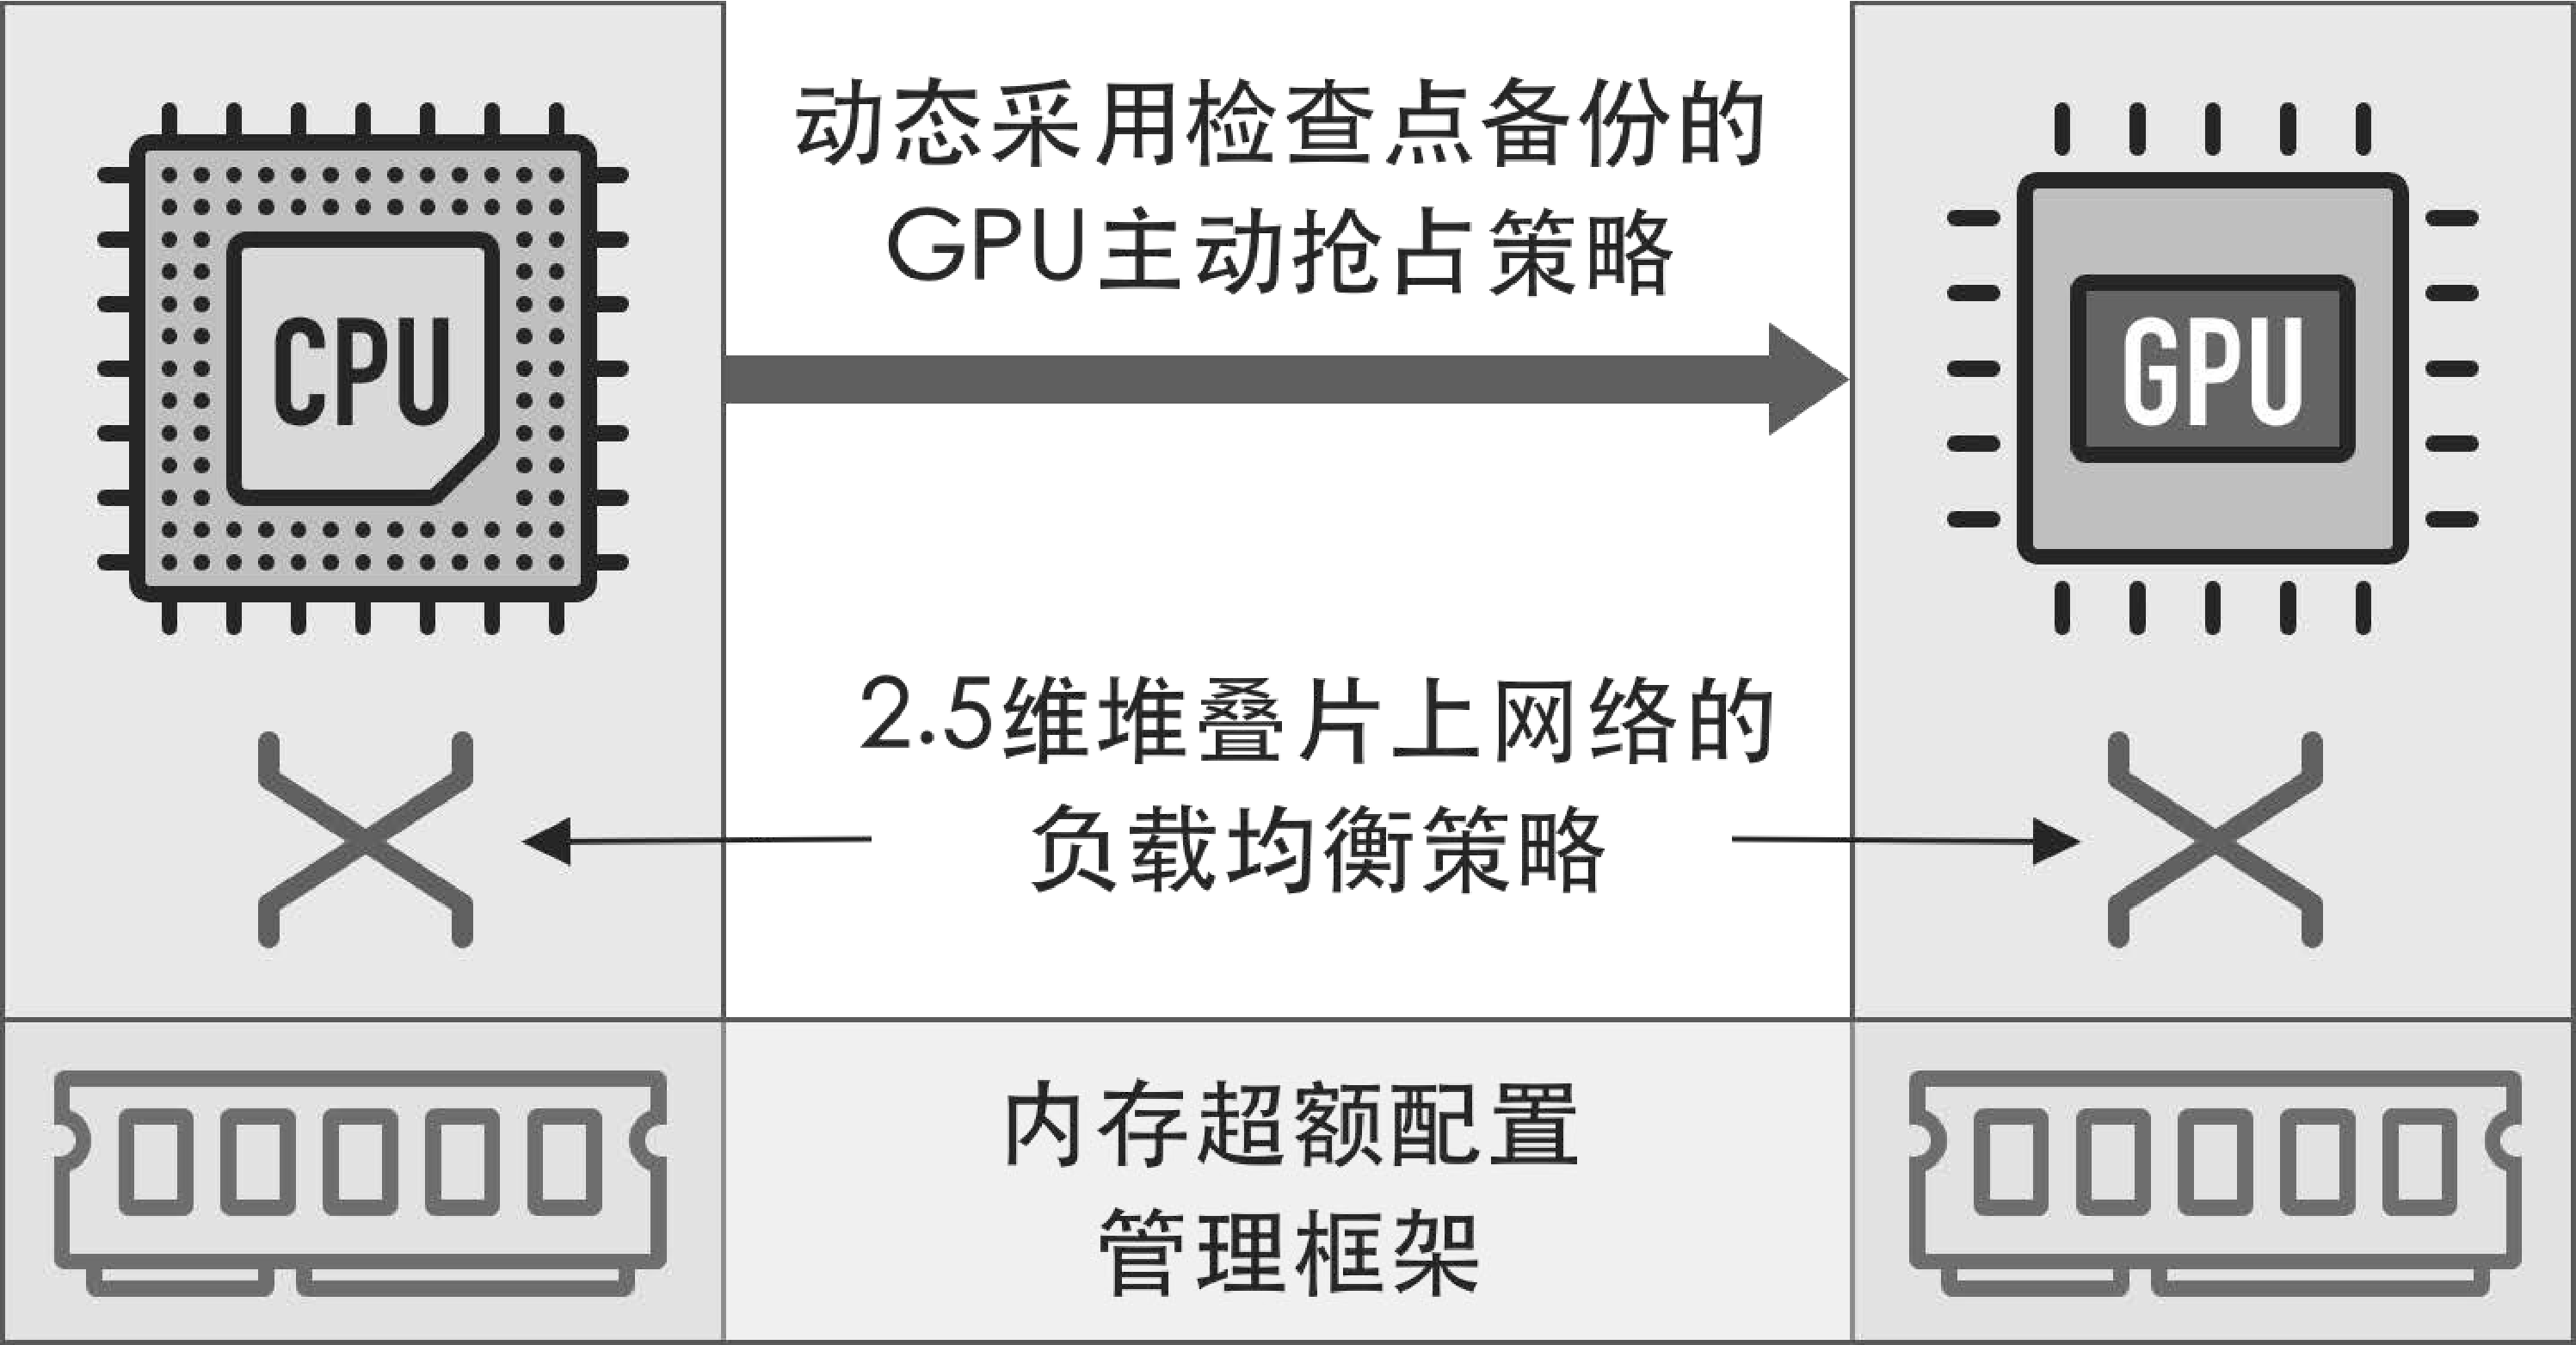
\includegraphics[width=\textwidth]{/Figs_Intro/structure}
  \caption{研究框架概述}
  \label{fig:structure}
\end{figure}

如图~\ref{fig:structure}所示,应用透明的软硬件策略包括:\texttt{面向CPU-GPU统一虚拟内存的内存超额配置管理框架},解决异构系统的内存超额配置问题;
\texttt{动态采用检查点备份的主动抢占策略},解决多任务切换时抢占延迟过高的问题;
以及\texttt{面向2.5维堆叠片上网络的负载均衡策略},解决两层网络负载不均衡的问题。
这三个研究点系统地分析了堆叠异构系统的内存管理、任务调度以及互连网络存在的问题,根据问题出现的原因提出了相应的应用透明解决策略。
应用透明的策略可以适应租户对数据中心系统运行不敏感的特点,在不增加程序员负担的同时,从软硬件结合的角度有效提升了异构系统的性能。


本文解决的三大问题主要位于堆叠异构系统的应用调度、网络和存储三部分。
这三部分相互独立,但并不冲突。
这些应用透明策略的共同应用,有助于缓解堆叠异构系统在不同层次的瓶颈,提升堆叠异构系统的性能。
在数据中心系统中,有助于优化多租户下的系统性能,同时对程序员的要求较低。




\section{论文组织结构}
本文紧紧围绕堆叠异构系统结构,对应用透明的架构和调度策略进行深入研究。
本文共分六章,按以下方式组织:
第~\ref{chap:intro}章为绪论,介绍了本文的研究动机以及相关研究内容和创新点;
第~\ref{chap:background}章从堆叠系统、GPU架构和异构系统相关策略优化三个方面介绍了本文的研究背景和相关基础;
第~\ref{chap:ETC}章介绍了针对GPU内存超额配置所提出的应用透明框架;
第~\ref{chap:PEP}章介绍了面向堆叠异构系统的多任务切换提出的基于动态检查点备份的优化方案;
第~\ref{chap:DLL}章介绍了针对2.5维堆叠片上网络结构提出的延迟感知的负载均衡策略;
第~\ref{chap:conclusion}章我们对全文进行了总结,并展望下一步工作。

\chapter{研究背景}
\label{chap:background}

\section{堆叠系统}

如今先进的三维堆叠芯片系统结构由于其在减少连线长度方面的天然优势,为减小未来芯片互连延迟和开销提供了非常有效的解决方案。
三维堆叠存储器的出现,能够为异构处理器提供更高的访存带宽,解决存储墙问题。
堆叠系统的这些优势使得我们有了许多为未来处理器体系结构提供创新设计的机会。

\subsection{三维堆叠集成}

%三维堆叠的基本概念和基本结构
三维堆叠封装技术属于最早的三维堆叠技术,是一种相对成熟的技术,已经在工业界得到了广泛应用。
三维堆叠封装技术通过\texttt{系统内集成封装(System-in-package, SiP)}或\texttt{封装内封装(Package-on-package, PoP)}技术将多个芯片垂直堆叠在一个基板上封装在一起,或者将多个封装号的芯片堆叠起来。
目前已经出现了许多成熟的采用三维封装技术的产品,包括在iPhone6中开始采用的Apple A8处理器,
将一个包含封装的双核CPU和4核GPU的处理器和一个1GB大小的LPDDR3 DRAM封装的存储器采用PoP技术封装在一起。
三维堆叠封装技术不要求在处理器结构和设计方法学上面做太大修改,因为这些技术的主要目标是为了节省空间,
芯片之间的通信仍然通过片外信号完成,因此无论是连接性和延迟都没有任何优势。

不同于三维堆叠封装技术,三维堆叠集成技术则是一种新兴技术。
三维堆叠集成技术将两或多层有源器件层,即CMOS晶体管层,在垂直方向上集成到一个芯片上。
堆叠芯片的层间提供了大量的互连资源,因此这种革命性的系统结构创新要求在设计方法学上的改变。
三维堆叠集成技术也可以分为两类:一类是\texttt{单晶堆叠方法(Monolithic Approach)},该方法在单一晶元上完成三维集成电路所有的设计制作流程,
最后将其切成晶粒。该方法只需要一个衬底,无需对准、削薄、粘接等流程。
另一类则是普通的堆叠方法,可以进一步被划分为\texttt{wafer-to-wafer}、\texttt{die-to-wafer}、和\texttt{die-to-die}等方法。这些方法都是在分别制造每一层的芯片,
最后被组装粘接组成三维堆叠芯片。不同于复杂的\texttt{单晶堆叠方法},不要求全新的设计制造技术,相对更加实际,也是三维集成电路技术的研究重点。


%三维堆叠的优势
相比于传统的集成电路技术,三维堆叠集成技术具有非常多的优势,我们从线长缩短、高访存带宽、异构集成和低成本四个角度介绍三维堆叠集成技术的优势:

\textbf{线长缩短}。芯片的全局连线延迟并没有按照摩尔定律的速度不断缩短,如今不断增加的全局连线延迟已经成为阻碍性能持续增长的重要原因之一。
三维堆叠集成技术能够有效克服全局连线延迟的瓶颈,为集成电路性能持续发展提供了解决方案。连线长度的缩减主要带来两方面巨大优势:延迟和功耗降低。
延迟的降低是由于平均线长和关键路径的缩短,而总线长的缩短也自然使得功耗大大降低。

\textbf{高存储带宽}。如今,如何为具有大量计算单元的GPU等异构处理器及时提供足够的数据已成为限制性能提升的重大挑战,因此提供高访存带宽尤为重要。
传统的片外存储单元由于受到I/O引脚的限制,难以提供足够的访存带宽。三维堆叠集成技术作为一种解决方案能为未来的微体系结构设计,特别是多核和众核处理器,
解决互连瓶颈、消除“存储墙”问题。通过将存储器堆叠在处理器芯片上,利用TSVs带来的通信优势提供远高于二维结构的通信带宽。

\textbf{异构集成}。三维堆叠集成技术为未来的体系结构设计提供了新的机会,即能够在新的维度进行设计空间探索。特别是异构集成能力,让我们从全新的角度研究系统结构的设计。
三维堆叠集成技术支持异构集成是由于其每一层都可以分开制造,不同的层也可以采用不同的工艺。
甚至可以在处理器层上堆叠光设备层、非易失性存储层或者是相变存储层,以实现高效异构系统结构。
这异构集成的实现可以为集成电路和芯片设计提供巨大的灵活性以满足性能、功耗和可靠性等要求。

\textbf{低成本}。随着集成电路规模不断增大,芯片的面积不断增大。但是由于缺陷密度相对恒定,较大的芯片晶粒大小意味着相对较低的良率。
而将多个较小的晶粒堆叠成一个相对较大规模的处理器增获得较高的良率,即使三维堆叠集成由于额外的制造复杂度可能会降低一定的良率。
另一方面,半导体集成电路的缩减也逐渐达到物理极限,继续缩减不但困难,成本也非常高。
因此三位堆叠集成技术潜在地提供了一种相比于传统集成电路更低成本的解决方案。


%三维堆叠的挑战
虽然三维堆叠集成技术带来了巨大的性能优势和在系统结构设计的机会,但在其广泛应用到未来的计算机系统前仍然需要解决几个重要的挑战:

\textbf{热问题}。功耗和热问题在传统的二维集成电路设计中已经成为一个重要的问题。
虽然三维堆叠集成技术相对于二维集成电路来说有许多的优势,然而将多个有源器件层堆叠起来大大增加了功耗密度,使得热问题进一步恶化,导致芯片温度升高。
芯片温度的升高又会反过来影响电路性能,如互连延迟会由于晶体管温度的升高而延长、静态功耗与温度是指数级依赖关系、温度升高还会导致热逃逸问题,此外,温度的升高会降低可靠性问题。

\textbf{设计工具和方法学}。如果没有辅助设计工具和方法学的支持,三维堆叠集成技术不可能商用化。
给定设计目标,高效的辅助设计工具和方法学可以帮助体系结构和电路设计者权衡三维堆叠电路在性能、功耗和开销。
相比于传统的二维集成电路,三维堆叠集成电路需要全新的布局规则,例如TSV布局、功耗计划等等。
高效的辅助设计工具还能够帮助分析热问题,在布局布线设计中避免热点区域的产生。

\textbf{测试问题}。在三维堆叠集成设计中,不同的测试策略和集成方法都可以严重影响系统的性能、功耗和开销问题。
三维堆叠集成电路技术目前没有广泛商用的另一个原因就是测试能力不足和缺乏面向三维堆叠集成技术的可测性设计技术。
如果没有在设计阶段考虑好测试问题,高效的三维集成测试时不可能的。
现在的三维堆叠集成测试上,一方面现在的探测技术不能够对所有的TSV进行探测;另一方面,测试过程很容易损坏被削薄的晶圆。



\subsection{基于硅中介层的2.5维堆叠}

三维堆叠集成技术可以将存储器直接堆叠在处理器晶圆之上。
不同于三维堆叠集成技术,2.5维堆叠策略的解决方案则是分别把存储器和处理器相邻地堆叠在硅中介层上,通过硅中介层的连线进行通信。
基于硅中介层的2.5维堆叠技术虽然是一代进化技术,但其能够在存储带宽和容量、热问题以及制造成本等方面表现出相对于三维堆叠集成技术更多的优势。

\textbf{存储容量和带宽}

对于三维堆叠集成,其主要优势是在两层间的最大潜在带宽受其面积限制。若采用直径50$\mu$s的TSV用作上下层的通信,
理论上一个200$cm^{2}$的芯片能够提供800万个TSVs。
相对地,对于2.5维堆叠集成,处理器和存储堆叠在硅中介层上的链接取决于处理器芯片的周长。
假设硅中介层上的连线直径也是50$\mu$s(全周长约56cm),则同样200$cm^{2}$的芯片仅能提供11000个连接点。
虽然三维堆叠和2.5维堆叠能提供的带宽有几个数量级的差异,但一个四通道的传统DDR3接口仅要求960个封装引脚。
硅中介层提供的成千上万的连接点已经可以避免这个瓶颈。
堆叠技术最重要的优势是将存储器和芯片封装在了一起,三维堆叠相对于2.5维堆叠更多的优势在这里实际并不明显。

而基于硅中介层的2.5维堆叠所能提供的存储容量则并不受限于处理器的面积,实际上能够堆叠在硅中介层上的堆叠存储的数目远远大于三维堆叠技术。
这是因为三维堆叠仅能从垂直方向上进行堆叠,受到了当前技术的限制。而硅中介层上的2.5维堆叠则能够支持多块堆叠存储水平分布,能够提供更大的存储容量。
当前的三维堆叠存储标准均为每块堆叠存储器提供了固定的带宽,因此总的存储带宽和容量取决于能够堆叠的存储器的数量。
对于当前的三维堆叠存储标准JEDEC HBM,提供1024位数据信号在1Gbps的平律师工作,每个堆叠存储能够提供128GB/s。 
而若4块HBM堆叠在硅中介层上,则总共能提供512GB/s的带宽。
假设一个HBM的大小为4GB,则基于硅中介层的2.5维堆叠能够提供16GB的存储容量,无论是带宽还是容量均优于三维堆叠技术。

\textbf{热问题}

基于硅中介层的2.5维堆叠相对于三维堆叠技术的另一个优势就是发热问题相对并不严重。
因为一般热问题比较严重的是处理器层,在2.5维堆叠技术上,处理器一般以单层的形式堆叠在硅中介层上,没有额外的层会堆叠在处理器上。
因此可以直接在处理器层上安装散热器。
当多块堆叠存储单元堆叠在硅中介层上时,温度虽然不会线性升高,但保持一个相对较低的温度依然对于降低刷新率和提高可靠性有重要意义。

\textbf{制造成本}

不同的堆叠技术要求不同的制造步骤,因此制造开销也会不一样。
基于硅中介层的2.5维堆叠技术相对于三维堆叠技术来说最明显的不同是2.5维堆叠技术需要增加额外的一个硅中介层的制造。
由于硅中介层需要更大的面积来堆叠更多的存储和处理器单元,且需要被削薄来支持TSV链接到C4 bumps。
因此硅中介层往往采用较老的一代半导体技术来实现。

三维堆叠结构的成本包括需要重新设计支持TSV的连接,这都是需要工程师的努力、EDA工具的支持、以及物理设计等。
同时TSV的面积和其周围的留空也需要为此增大芯片的面积。
而2.5维堆叠技术在处理器层不需要TSV,因此芯片无需削薄和面积的增大。

虽然2.5维堆叠和3维堆叠解决方案之间还有许多可以比较的优缺点,但根据上述的主要问题,我们认为2.5维堆叠技术对于异构系统来说非常令人期待。
堆叠异构系统采用2.5维堆叠技术可以获得更高的存储带宽和更大的存储容量,同时在热管理上也有更多的优势。
因此,本文研究的堆叠异构系统也主要基于2.5维堆叠技术,研究其在内存墙问题、多任务切换问题和网络负载均衡上的问题,并提供解决方案。

\section{GPU架构与编程模型}

\subsection{GPU架构}

\subsection{GPU编程模型}


\section{异构系统的策略优化}

\subsection{软件策略优化}

\subsection{硬件策略优化}

















% 本章将进入论文排版的正文, 按元素分主要包括:
% {\kai 字体段落,图片表格,公式定理,参考文献}这几部分。
% 这个样例文件将包括模板中使用到的所有格式、模板中自定义命令到或者特有的东西,
% 都将被一一介绍,希望大家在排版自己的学位论文前能细致的看一遍,记住样例的格式和
% 方法,方便上手。

% \section{字体段落}
% \label{sec:font}

% 陈赓(1903年2月27日-1961年3月16日),原名陈庶康,中国湖南湘乡人,军事家。出生将门,其祖父为湘军将领陈翼怀。

% Adobe中文字体有四种:

% {\kai 楷体\verb|\kai|:陈赓,中国湖南湘乡人,军事家。出生将门,其祖父为湘军将领陈翼怀。%
% 1952年筹办并任人民解放军军事工程学院第一任院长兼政委,培养国防科技人才。1955年被授予大将军衔。}

% {\fs 仿宋\verb|\fs|:陈赓,中国湖南湘乡人,军事家。出生将门,其祖父为湘军将领陈翼怀。%
% 1952年筹办并任人民解放军军事工程学院第一任院长兼政委,培养国防科技人才。1955年被授予大将军衔。}

% {\hei 黑体\verb|\hei|:陈赓,中国湖南湘乡人,军事家。出生将门,其祖父为湘军将领陈翼怀。%
% 1952年筹办并任人民解放军军事工程学院第一任院长兼政委,培养国防科技人才。1955年被授予大将军衔。}

% 宋体就是正文字体了。下面测试字体大小,\LaTeX{}默认的列表环境会在
% 条目之间插入过多的行距,在下面这种情况可能正好,若用户需要
% {\kai 正文行距}的列表环境,可以使用compactitem环境,记住这点很重要,不要再
% 用那种自己修改\verb|itemsep|的傻傻的办法了。
% \begin{itemize}
% \item[初号] {\song\chuhao 陈赓大将}
% \item[小初] {\song\xiaochu 陈赓大将}
% \item[一号] {\song\yihao 陈赓大将}
% \item[小一] {\song\xiaoyi 陈赓大将}
% \item[二号] {\song\erhao 陈赓大将}
% \item[小二] {\song\xiaoer 陈赓大将}
% \item[三号] {\song\sanhao 陈赓大将}
% \item[小三] {\song\xiaosan 陈赓大将}
% \item[四号] {\song\sihao 陈赓大将}
% \item[小四] {\song\xiaosi 陈赓大将}
% \item[五号] {\song\wuhao 陈赓大将}
% \item[小五] {\song\xiaowu 陈赓大将}
% \end{itemize}

% \section{表格明细}
% \label{sec:figure}
% 表格是论文的重要组成部分,我们从简单的表格讲起,到复杂的表格为止。

% 模板中关于表格的宏包有三个: \textsf{booktabs}、\textsf{array} 和
% \textsf{longtabular}。三线表建议使用\textsf{booktabs}中提供的,
% 包含toprule、midrule 和 bottomrule三条命令,简单干脆!
% 它们与\textsf{longtable} 能很好的配合使用。下面来看一个表格实例:
% \begin{table}[htb]
%   \centering
%   \begin{minipage}[t]{0.8\linewidth} % 如果想在表格中使用脚注,minipage是个不错的办法
%   \caption[模板文件]{模板文件。如果表格的标题很长,那么在表格索引中就会很不美
%     观,所以要像 chapter 那样在前面用中括号写一个简短的标题。这个标题会出现在索
%     引中。}
%   \label{tab:template-files}
%     \begin{tabular*}{\linewidth}{lp{10cm}}
%       \toprule[1.5pt]
%       {\hei 文件名} & {\hei 描述} \\
%       \midrule[1pt]
%       nudtpaper.ins & \LaTeX{} 安装文件,docstrip\footnote{表格中的脚注} \\
%       nudtpaper.dtx & 所有的一切都在这里面\footnote{再来一个}。\\
%       nudtpaper.cls & 模板类文件。\\
%       nudtpaper.cfg & 模板配置文。cls 和 cfg 由前两个文件生成。\\
%       bstutf8.bst   & 参考文献 Bibtex 样式文件。\\
%       mynudt.sty    & 常用的包和命令写在这里,减轻主文件的负担。\\
%       \bottomrule[1.5pt]
%     \end{tabular*}
%   \end{minipage}
% \end{table}

% 表 \ref{tab:template-files} 列举了本模板主要文件及其功能,基本上来说论文
% 中最可能用到的就是这种表格形式了。
% 请大家注意三线表中各条线对应的命令。这个例子还展示了如何在表格中正确使用脚注。
% 如果你不需要在表格中插入脚注,可以将minipage环境去掉。
% 由于\LaTeX{}本身不支持在表格中使用\verb|\footnote|,所以我们不得不将表格放在
% 小页中,而且最好将表格的宽度设置为小页的宽度,这样脚注看起来才更美观。

% 另外六院的同学在使用模板时需要使用一种固定宽度(往往是页宽,下面的例子由
% rongdonghu提供)的表格,内容需要居中且可以自动调整。
% 解决办法是自定义了一种\verb|tabularx|中的\textbf{Z}环境,在论文模板中,
% 该命令已添加到\verb|mynudt.sty|中。下面是这种情况的实例:

% \begin{table}[htbp]
% \centering
% \begin{minipage}[t]{0.9\linewidth}
% \caption{Reed Solomon码的典型应用}
% \label{tab:RSuse}
% \begin{tabularx}{\linewidth}{cZ}
% \toprule[1.5pt]
% {\hei 应用领域} & {\hei 编码方案}\\
% \midrule[1pt]
% 磁盘驱动器 & RS(32,28,5)码 \footnote{码长为32、维数为28、最小距离为5} \\
% CD & 交叉交织RS码(CIRC) \\
% DVD & RS(208,192,17)码、RS(182,172,11)码 \\
% 光纤通信 & RS(255,229,17)码 \\
% \bottomrule[1.5pt]
% \end{tabularx}
% \end{minipage}
% \end{table}

% 我们经常会在表格下方标注数据来源,或者对表格里面的条目进行解释。前面的脚注是一种
% 不错的方法,如果你不喜欢minipage方法的脚注。
% 那么完全可以在表格后面自己写注释,比如表~\ref{tab:tabexamp1}。
% \begin{table}[htbp]
%   \centering
%   \caption{复杂表格示例 1}
%   \label{tab:tabexamp1}
%   \begin{minipage}[t]{0.8\textwidth} 
%     \begin{tabularx}{\linewidth}{|l|X|X|X|X|}
%       \hline
%       \multirow{2}*{\backslashbox{x}{y}}  & \multicolumn{2}{c|}{First Half} & \multicolumn{2}{c|}{Second Half}\\
%       \cline{2-5}
%       & 1st Qtr &2nd Qtr&3rd Qtr&4th Qtr \\ 
%       \hline
%       \multirow{2}*{East$^{*}$} &   20.4&   27.4&   90&     20.4 \\
%        &   30.6 &   38.6 &   34.6 &  31.6 \\ 
%       West$^{**}$ &   30.6 &   38.6 &   34.6 &  31.6 \\ 
%       \hline
%     \end{tabularx}\\[2pt]
%     \footnotesize
%     *:东部\\
%     **:西部
%   \end{minipage}
% \end{table}

% 此外,表~\ref{tab:tabexamp1} 同时还演示了另外三个功能:1)通过 \textsf{tabularx} 的
%  \texttt{|X|} 扩展实现表格内容自动调整;2)通过命令 \verb|\backslashbox| 在表头部分
% 插入反斜线(WORD中很简单,但\LaTeX{}做表格需要一定的(极大的)想象力);3)就是
% 使用\verb|multirow|和\verb|multicolumn|命令。

% 不可否认 \LaTeX{} 的表格功能没有想象中的那么强大,不过只要你足够认真,足够细致,那么
% 同样可以排出来非常复杂非常漂亮的表格。可是科技论文中那么复杂表格有什么用呢?
% 上面那个表格就够用啦。

% 浮动体的并排放置一般有两种情况:1)二者没有关系,为两个独立的浮动体;2)二者隶属
% 于同一个浮动体。对表格来说并排表格既可以像表~\ref{tab:parallel1}、表~\ref{tab:parallel2} 
% 使用小页环境,也可以如表~\ref{tab:subtable}使用子表格来做。
% 图与表同出一源,后面我们将讲解子图(subfloat)的例子。
% \begin{table}[htb]
% \centering
% \noindent\begin{minipage}{0.45\textwidth}
% \centering
% \caption{第一个并排子表格}
% \label{tab:parallel1}
% \begin{tabular}{p{2cm}p{2cm}}
% \toprule[1.5pt]
% 111 & 222 \\\midrule[1pt]
% 222 & 333 \\\bottomrule[1.5pt]
% \end{tabular}
% \end{minipage}
% \begin{minipage}{0.45\textwidth}
% \centering
% \caption{第二个并排子表格}
% \label{tab:parallel2}
% \begin{tabular}{p{2cm}p{2cm}}
% \toprule[1.5pt]
% 111 & 222 \\\midrule[1pt]
% 222 & 333 \\\bottomrule[1.5pt]
% \end{tabular}
% \end{minipage}
% \end{table}
% \begin{table}[htbp]
% \centering
% \caption{并排子表格}
% \label{tab:subtable}
% \subfloat[第一个子表格]{
% \begin{tabular}{p{2cm}p{2cm}}
% \toprule[1.5pt]
% 111 & 222 \\\midrule[1pt]
% 222 & 333 \\\bottomrule[1.5pt]
% \end{tabular}}\hskip2cm
% \subfloat[第二个子表格]{
% \begin{tabular}{p{2cm}p{2cm}}
% \toprule[1.5pt]
% 111 & 222 \\\midrule[1pt]
% 222 & 333 \\\bottomrule[1.5pt]
% \end{tabular}}
% \end{table}

% 如果您要排版的表格长度超过一页,那么推荐使用\textsf{longtable}命令。
% 这里随便敲入一些无关的文字,使得正文看上去不是那么的少。
% 表~\ref{tab:performance} 就是 \textsf{longtable} 的简单示例。
% \begin{longtable}[c]{c*{6}{r}}
% \caption{实验数据}\label{tab:performance}\\
% \toprule[1.5pt]
%  测试程序 & \multicolumn{1}{c}{正常运行} & \multicolumn{1}{c}{同步}
% & \multicolumn{1}{c}{检查点}   & \multicolumn{1}{c}{卷回恢复}
% & \multicolumn{1}{c}{进程迁移} & \multicolumn{1}{c}{检查点} 	\\
% & \multicolumn{1}{c}{时间 (s)} & \multicolumn{1}{c}{时间 (s)}
% & \multicolumn{1}{c}{时间 (s)} & \multicolumn{1}{c}{时间 (s)}
% & \multicolumn{1}{c}{时间 (s)} &  文件(KB)			\\
% \midrule[1pt]%
% \endfirsthead%

% \multicolumn{7}{c}{续表~\thetable\hskip1em 实验数据}\\

% \toprule[1.5pt]
%  测试程序 & \multicolumn{1}{c}{正常运行} & \multicolumn{1}{c}{同步} 
% & \multicolumn{1}{c}{检查点}   & \multicolumn{1}{c}{卷回恢复}
% & \multicolumn{1}{c}{进程迁移} & \multicolumn{1}{c}{检查点} 	\\
% & \multicolumn{1}{c}{时间 (s)} & \multicolumn{1}{c}{时间 (s)}
% & \multicolumn{1}{c}{时间 (s)} & \multicolumn{1}{c}{时间 (s)}
% & \multicolumn{1}{c}{时间 (s)} &  文件(KB)			\\
% \midrule[1pt]%
% \endhead%
% \hline%

% \multicolumn{7}{r}{续下页}%

% \endfoot%
% \endlastfoot%
% CG.A.2 & 23.05   & 0.002 & 0.116 & 0.035 & 0.589 & 32491  \\
% CG.A.4 & 15.06   & 0.003 & 0.067 & 0.021 & 0.351 & 18211  \\
% CG.A.8 & 13.38   & 0.004 & 0.072 & 0.023 & 0.210 & 9890   \\
% CG.B.2 & 867.45  & 0.002 & 0.864 & 0.232 & 3.256 & 228562 \\
% CG.B.4 & 501.61  & 0.003 & 0.438 & 0.136 & 2.075 & 123862 \\
% CG.B.8 & 384.65  & 0.004 & 0.457 & 0.108 & 1.235 & 63777  \\
% MG.A.2 & 112.27  & 0.002 & 0.846 & 0.237 & 3.930 & 236473 \\
% MG.A.4 & 59.84   & 0.003 & 0.442 & 0.128 & 2.070 & 123875 \\
% MG.A.8 & 31.38   & 0.003 & 0.476 & 0.114 & 1.041 & 60627  \\
% MG.B.2 & 526.28  & 0.002 & 0.821 & 0.238 & 4.176 & 236635 \\
% MG.B.4 & 280.11  & 0.003 & 0.432 & 0.130 & 1.706 & 123793 \\
% MG.B.8 & 148.29  & 0.003 & 0.442 & 0.116 & 0.893 & 60600  \\
% LU.A.2 & 2116.54 & 0.002 & 0.110 & 0.030 & 0.532 & 28754  \\
% LU.A.4 & 1102.50 & 0.002 & 0.069 & 0.017 & 0.255 & 14915  \\
% LU.A.8 & 574.47  & 0.003 & 0.067 & 0.016 & 0.192 & 8655   \\
% LU.B.2 & 9712.87 & 0.002 & 0.357 & 0.104 & 1.734 & 101975 \\
% LU.B.4 & 4757.80 & 0.003 & 0.190 & 0.056 & 0.808 & 53522  \\
% LU.B.8 & 2444.05 & 0.004 & 0.222 & 0.057 & 0.548 & 30134  \\
% EP.A.2 & 123.81  & 0.002 & 0.010 & 0.003 & 0.074 & 1834   \\
% EP.A.4 & 61.92   & 0.003 & 0.011 & 0.004 & 0.073 & 1743   \\
% EP.A.8 & 31.06   & 0.004 & 0.017 & 0.005 & 0.073 & 1661   \\
% EP.B.2 & 495.49  & 0.001 & 0.009 & 0.003 & 0.196 & 2011   \\
% EP.B.4 & 247.69  & 0.002 & 0.012 & 0.004 & 0.122 & 1663   \\
% EP.B.8 & 126.74  & 0.003 & 0.017 & 0.005 & 0.083 & 1656   \\
% \bottomrule[1.5pt]
% \end{longtable}

% 另外,有的同学不想让某个表格或者图片出现在索引里面,那么请使用命令 \verb|\caption*{}|,
% 这个命令不会给表格编号,也就是出来的只有标题文字而没有“表~XX”,“图~XX”,否则
% 索引里面序号{\kai 不连续}就显得不伦不类,这也是 \LaTeX{} 里星号命令默认的规则。

% \section{绘图插图}

% 本模板不再预先装载任何绘图包(如 \textsf{pstricks,pgf} 等),完全由你自己来决定。
% 个人觉得 \textsf{pgf} 不错,不依赖于 Postscript。此外还有很多针对 \LaTeX{} 的
%  GUI 作图工具,如 XFig(jFig), WinFig, Tpx, Ipe, Dia, Inkscape, LaTeXPiX,
% jPicEdt 等等。本人强烈推荐\textsf{Ipe}。

% 一般图形都是处在浮动环境中。之所以称为浮动是指最终排版效果图形的位置不一定与源文
% 件中的位置对应,这也是刚使用 \LaTeX{} 同学可能遇到的问题。
% 如果要强制固定浮动图形的位置,请使用 \textsf{float} 宏包,
% 它提供了 \texttt{[H]}(意思是图片就给我放在这里\textcolor{red}{H}ere)参数,
% 但是除非特别需要,不建议使用\texttt{[H]},而是推荐使用\texttt{[htbp]},
% 给\LaTeX{}更多选择。比如图~\ref{fig:ipe}。
% \begin{figure}[htbp] % use float package if you want it here
%   \centering
%   \includegraphics[width=3in]{hello}
%   \caption{利用IPE制图}
%   \label{fig:ipe}
% \end{figure}

% 若子图共用一个计数器,
% 那么请看图~\ref{fig:big1},它包含两个小图,分别是图~\ref{fig:subfig1} 
% 和图~\ref{fig:subfig2}。这里推荐使用\verb|\subfloat|,{\bf 不要再用}
% \verb|\subfigure|和\verb|\subtable|。
% \begin{figure}[htb]
%   \centering%
%   \subfloat[第一个小图形]{%
%     \label{fig:subfig1}
%     \includegraphics[height=2cm]{xh}}\hspace{4em}%
%   \subfloat[第二个小图形。如果标题很长的话,它会自动换行,这个 caption 就是这样的例子]{%
%     \label{fig:subfig2}
%     \includegraphics[height=2cm]{xhh}}
%   \caption{包含子图形的大图形}
%   \label{fig:big1}
% \end{figure}

% 而下面这个例子显示并排$3\times2$的图片,见图\ref{fig:subfig:3x2}:
% \begin{figure}[htb]
% \centering
% \subfloat[]{\includegraphics[width=.27\textwidth]{typography}} \qquad
% \subfloat[]{\includegraphics[width=.27\textwidth]{typography}} \qquad
% \subfloat[]{\includegraphics[width=.27\textwidth]{typography}} \qquad
% \subfloat[]{\includegraphics[width=.27\textwidth]{typography}} \qquad
% \subfloat[]{\includegraphics[width=.27\textwidth]{typography}} \qquad
% \subfloat[]{\includegraphics[width=.27\textwidth]{typography}}
% \caption{并排图片}
% \label{fig:subfig:3x2}
% \end{figure}

% 要注意,图\ref{fig:subfig:3x2}例中
% \texttt{qquad}相当于\verb|\hspace{2em}|,也就是2个字符的宽度,约0.08倍页宽,
% 图片宽度设定为0.27倍页宽是合适的;在该环境中,尽量不要手动换行,所以,不妨自己计算一下!

% 如果要把编号的两个图形并排,那么小页(minipage)就非常有用了,可以分别参考
% 图\ref{fig:parallel1}和图\ref{fig:parallel2}。其实这个例子和表格一节中并排
% 放置的表格一摸一样。
% \begin{figure}[htb]
% \begin{minipage}{0.48\textwidth}
%   \centering
%   \includegraphics[height=1.2cm]{xhh}
%   \caption{并排第一个图}
%   \label{fig:parallel1}
% \end{minipage}\hfill
% \begin{minipage}{0.48\textwidth}
%   \centering
%   \includegraphics[height=1.2cm]{xhh}
%   \caption{并排第二个图}
%   \label{fig:parallel2}
% \end{minipage}
% \end{figure}

% 图形就说这么多,因为大家在写论文是遇到的最大问题不是怎么把图插进去,
% 而是怎样做出专业的、诡异的、震撼的图片来,记得在这时参考前面推荐的那
% 些工具吧,当然必不可少的是Matlab了,至于如何加入中文标注、支持中文等等
% 可以上网去查,但这里{\kai 推荐一点},用好export命令,使得插入图片时尽可能的不要
% 缩放,保证图文的一致性。

% \section{公式定理}
% \label{sec:equation}
% 贝叶斯公式如式~(\ref{equ:chap1:bayes}),其中$p(y|\mathbf{x})$为后验;
% $p(\mathbf{x})$为先验;分母$p(\mathbf{x})$ 为归一化因子,这是
% 实际应用中十分恐怖的一个积分式。
% \begin{equation}
% \label{equ:chap1:bayes}
% p(y|\mathbf{x}) = \frac{p(\mathbf{x},y)}{p(\mathbf{x})}=
% \frac{p(\mathbf{x}|y)p(y)}{p(\mathbf{x})} 
% \end{equation}

% 论文里面公式越多,\TeX{} 就越 happy。再看一个 \textsf{amsmath} 的例子:
% \newcommand{\envert}[1]{\left\lvert#1\right\rvert} 
% \begin{equation}\label{detK2}
% \det\mathbf{K}(t=1,t_1,\dots,t_n)=\sum_{I\in\mathbf{n}}(-1)^{\envert{I}}
% \prod_{i\in I}t_i\prod_{j\in I}(D_j+\lambda_jt_j)\det\mathbf{A}
% ^{(\lambda)}(\overline{I}|\overline{I})=0.
% \end{equation} 

% 大家在写公式的时候一定要好好看\textsf{amsmath}的文档,并参考模板中的用法:
% \begin{multline*}%\tag{[b]} % 这个出现在索引中的
% \int_a^b\biggl\{\int_a^b[f(x)^2g(y)^2+f(y)^2g(x)^2]
%  -2f(x)g(x)f(y)g(y)\,dx\biggr\}\,dy \\
%  =\int_a^b\biggl\{g(y)^2\int_a^bf^2+f(y)^2
%   \int_a^b g^2-2f(y)g(y)\int_a^b fg\biggr\}\,dy
% \end{multline*}

% 再看\ref{equ:split}:
% \begin{equation}\label{equ:split}
% \begin{split}
% C(z) &= [z^n] \biggl[\frac{e^{3/4}}{\sqrt{1-z}} +
% e^{-3/4}(1-z)^{1/2} + \frac{e^{-3/4}}{4}(1-z)^{3/2}
% + O\Bigl( (1-z)^{5/2}\Bigr)\biggr] \\
% &= \frac{e^{-3/4}}{\sqrt{\pi n}} - \frac{5e^{-3/4}}{8\sqrt{\pi
% n^3}} + \frac{e^{-3/4}}{128 \sqrt{\pi n^5}} +
% O\biggl(\frac{1}{\sqrt{\pi
% n^7}}\biggr)
% \end{split}
% \end{equation}

% 当然了,数学中必不可少的是定理和证明:
% \begin{theorem}
%   \label{chapTSthm:rayleigh solution}
%   假定 $X$ 的二阶矩存在:
%   \begin{equation}
%          O_R(\mathbf{x},F)=\sqrt{\frac{\mathbf{u}_1^T\mathbf{A}\mathbf{u}_1} {\mathbf{u}_1^T\mathbf{B}\mathbf{u}_1}}=\sqrt{\lambda_1},
%   \end{equation}
%   其中 $\mathbf{A}$ 等于 $(\mathbf{x}-EX)(\mathbf{x}-EX)^T$,$\mathbf{B}$ 表示协方差阵 $E(X-EX)(X-EX)^T$,$\lambda_1$
% $\mathbf{u}_1$是$\lambda_1$对应的特征向量,
% \end{theorem}

% 对于希腊符号使用\verb|mathbf|命令可能有些问题,所以建议对符号
% 用\verb|bm|加粗,记得用\verb|\up<greek>|切换正体符号,下面看几个例子:
% \verb|\gamma|斜体代表变量$\gamma$,\verb|\bm{\upgamma}|正体代表向量$\bm{\upgamma}$,
% 。\verb|\Gamma|正体代表操作符号$\Gamma$,
% \verb|\bm{\Gamma}|正体粗体代表矩阵形式$\bm{\Gamma}$,
% \verb|\varGamma|斜体代表变量$\varGamma$。另外对于大小写斜体的加粗可以见$\bm{\gamma}$和$\bm{\varGamma}$,
% 但是这两种科技论文中很少出现,这里只做测试。
% 非符号普通向量就用\verb|\mathbf|吧:$\mathbf{x}_k,\mathbf{X}_k$。
% 完整测试如下$\omega,\bm{\omega},\upomega,\bm{\upomega},\Omega,\bm{\Omega},\varOmega,\bm{\varOmega}$。

% \begin{proof}
% 上述优化问题显然是一个Rayleigh商问题。我们有
%   \begin{align}
%      O_R(\mathbf{x},F)=\sqrt{\frac{\mathbf{u}_1^T\mathbf{A}\mathbf{u}_1} {\mathbf{u}_1^T\mathbf{B}\mathbf{u}_1}}=\sqrt{\lambda_1},
%  \end{align}
%  其中 $\lambda_1$ 下列广义特征值问题的最大特征值:
% $$
% \mathbf{A}\mathbf{z}=\lambda\mathbf{B}\mathbf{z}, \mathbf{z}\neq 0.
% $$
%  $\mathbf{u}_1$ 是 $\lambda_1$对应的特征向量。结论成立。
% \end{proof}

% 下面来看看算法环境的定义和使用。
% 我们知道,故障诊断的最终目的,是将故障定位到部件,而由于信号--部件依赖矩阵的存在,因此,实质性的工作是找出由故障部件发出异常信号,
% 不妨称为源异常信号,而如前所述,源异常信号与异常信号依赖矩阵$\mathbf{S_a}$的全零列是存在一一对应的关系的。因此,我们只要获得了$\mathbf{S_a}$的全零列的相关信息,
% 也就获得了源异常信号的信息,从而能进一步找到故障源。
% 通过以上分析,我们构造算法\ref{alg53},用于实现非回路故障诊断。
% \begin{algorithm}[htbp]
%   \caption{非回路故障诊断算法}
%   \label{alg53}
%   \begin{algorithmic}[1]
%     \REQUIRE 信号--部件依赖矩阵$\mathbf{A}$,信号依赖矩阵$\mathbf{S}$,信号状态向量$\alpha$
%     \ENSURE 部件状态向量$\gamma$
%     \STATE $\mathbf{P}\leftarrow\left(<\alpha>\right)$
%     \STATE $\mathbf{S_{a}}\leftarrow\mathbf{P^T}\mathbf{S}\mathbf{P}$
%     \FOR{$i=1$ to $S_a$的阶数$m$}
%     \STATE $s_i\leftarrow s_i$的第$i$个行向量
%     \ENDFOR
%     \STATE $\beta_a\leftarrow\lnot \left(s_1\lor s_2\lor \cdots\lor s_m\right)^T$
%     \STATE $\beta\leftarrow\mathbf{P}\beta_a$
%     \STATE $\gamma\leftarrow\mathbf{A}\beta$
%   \end{algorithmic}
% \end{algorithm}

% 第一类故障回路推理与非回路故障推理是算法基本相同,稍微不同的是$\beta_a$的计算。因为第一类故障回路中的信号全部可能是源异常信号,因此我们不必计算
% $\beta_a=\lnot \left(\left[s_1\lor s_2\lor \cdots\lor s_m\right]^T\right)$,而直接取$\beta_a=\underbrace{\left[\begin{array}{cccc}1&1&\cdots&1\end{array}\right]^T}_m$,将$\beta_a$代入
% 算法\ref{alg53},有
% \[\beta=\mathbf{P}\beta_a=\mathbf{P}\underbrace{\left[\begin{array}{cccc}1&1&\cdots&1\end{array}\right]^T}_m=\alpha\]
% 因此一类故障回路的推理算法变得相当简单,例如算法\ref{alg54}
% \begin{algorithm}[htbp]
%   \caption{第一类故障回路诊断算法}
%   \label{alg54}
%   \begin{algorithmic}[1]
%     \REQUIRE 信号--部件依赖矩阵$\mathbf{A}$,信号状态向量$\alpha$
%     \ENSURE 部件状态向量$\gamma$
%     \STATE $\gamma\leftarrow\mathbf{A}\alpha$
%   \end{algorithmic}
% \end{algorithm}

% \section{参考文献}
% \label{sec:bib}
% 当然参考文献可以直接写 bibitem,虽然费点功夫,但是好控制,各种格式可以自己随意改
% 写,在nudtpaper里面,建议使用JabRef编辑和管理文献,再结合\verb|bstutf8.bst|,
% 对中文的支持非常不错,格式也很规范。

% 本模板推荐使用 BIB\TeX,样式文件为 bstutf8.bst,符合学校的参考文献格式(如专利
% 等引用未加详细测试)。看看这个例子,关于书的\upcite{tex, companion},
% 还有这些\upcite{Krasnogor2004e, clzs, zjsw},关于杂志的\upcite{ELIDRISSI94,
%   MELLINGER96, SHELL02},硕士论文\upcite{zhubajie, metamori2004},博士论文
% \upcite{shaheshang, FistSystem01},标准文件\upcite{IEEE-1363},会议论文\upcite{DPMG,kocher99},%
% 技术报告\upcite{NPB2}。中文参考文献\upcite{cnarticle}\textsf{特别注意},需要在\verb|bibitem|中
% 增加\verb|language|域并设为\verb|zh|,英文此项可不填,之后由\verb|bstutf8|统一处理
% (具体就是决定一些文献在中英文不同环境下的显示格式,如等、etc)。
% 若使用\verb|JabRef|,则你可按下面步骤来设置:
% 选择\textsf{Options}$\rightarrow$\textsf{Set Up General Fields},
% 在\verb|General:|后加入\verb|language|就可以了。

% 有时候不想要上标,那么可以这样 \cite{shaheshang},这个非常重要。

% \section{代码高亮}
% 有些时候我们需要在论文中引入一段代码,用来衬托正文的内容,或者体现关键思路的实现。
% 在模板中,统一使用\texttt{listings}宏包,并且设置了基本的内容格式,并建议用户只
% 使用三个接口,分别控制:编程语言,行号以及边框。简洁达意即可,下面分别举例说明。

% 首先是设定语言,来一个C的,使用的是默认设置:
% \begin{lstlisting}[language=C]
% void sort(int arr[], int beg, int end)
% {
%   if (end > beg + 1)
%   {
%     int piv = arr[beg], l = beg + 1, r = end;
%     while (l < r)
%     {
%       if (arr[l] <= piv)
%         l++;
%       else
%         swap(&arr[l], &arr[--r]);
%     }
%     swap(&arr[--l], &arr[beg]);
%     sort(arr, beg, l);
%     sort(arr, r, end);
%   }
% }
% \end{lstlisting}

% 当我们需要高亮Java代码,不需要行号,不需要边框时,可以:
% \begin{lstlisting}[language=Java,numbers=none,frame=none]
% // A program to display the message
% // "Hello World!" on standard output

% public class HelloWorld {
 
%    public static void main(String[] args) {
%       System.out.println("Hello World!");
%    }
      
% }   // end of class HelloWorld
% \end{lstlisting}

% 细心的用户可能发现,行号被放在了正文框之外,事实上这样是比较美观的,
% 如果有些用户希望在正文框架之内布置所有内容,可以:
% \begin{lstlisting}[language=perl,xleftmargin=2em,framexleftmargin=1.5em]
% #!/usr/bin/perl
% print "Hello, world!\n";
% \end{lstlisting}

% 好了,就这么多,\texttt{listings}宏包的功能很强大也很复杂,如果需要自己定制,
% 可以查看其手册,耐心阅读总会找到答案。
% \textbf{注意:} 当前代码环境中文注释的处理还不是很完善,对于注释请妥善处理。
% 在本模板中,推荐算法环境或者去掉中文的listings代码环境。
% 如果需要包含中文注释,不要求代码高亮,
% 就用\texttt{code}环境,这个环境是Verbatim的定制版,简单有效,
% 调用的是fancyvbr宏包,用户可在mynudt.sty中修改它的外观等等。
% 这里我们还可以给代码加上标签。
% \begin{code}[label=hello.c]
% public class HelloWorld {
%    public static void main(String[] args) {
%       System.out.println("Hello World!");
%    }
% }   // 世界,你好!
% \end{code}

% \section{符号列表}

% {\hei 前面的话:}{\kai\color{blue} 
% 2.2版本后默认使用nomencl环境,如果你还是希望使用传统的\verb|definition.tex|,那么只需注释掉
% 顶层文件中的nomenclature即可。}

% 符号列表使用的是\verb|nomencl|包,自己简单定制了下,使用方法分为四步:
% \begin{compactenum}
% \item 将\verb|\makenomenclature|语句放在正文前,即\verb|\begin{document}|前面;
% \item 将\verb|\printnomenclature|放在论文中,我在例子中将符号列表放在了英文摘要的
% 后面,正文第一章的前面,当然,你可以根据自己的需要或者教研室的规范放置在合理的位置上,
% 为了页面引用的正确,在这句话前面放上\verb|\cleardoublepage|;
% \item 使用\verb|\nomenclature|命令在论文的各个位置上添加符号定义,语法后面会讲到;
% \item 编译。编译需要首先运行一遍xelatex,之后运行
% \begin{code}
% makeindex -s nomencl.ist -o thesis.nls thesis.nlo
% \end{code}
% \end{compactenum}

% 你可以把这句编译命令放在\verb|makepdf.bat|中第一个\verb|xelatex thesis|下面。然后
% 双击\verb|makepdf.bat|就可以了,论文模板中已经为你添加上了,如果你强烈不想使用
% nomencl环境,只要把它注释掉(前面加\verb|rem|)就可以。
% 另外,由于我使用的是VIM来编辑\TeX{}代码,具体到每个编辑器(诸如WinEDT,TeXWorks等)
% 如何设定该命令的快捷按钮,诸位可以搜索网上的教程。

% 下面简单说明下\verb|\nomenclature|命令,语法为。这里插入一些随机的文字,希望
% 对你在阅读帮助中的思维没有什么不良的影响。
% \begin{code}
% \nomenclature[<prefix>]{<symbol>}{<desc>}{<null>}
% \end{code}
% \verb|nomencl|模板的默认排序方法可能(大多都)不满足要求,
% 论文模板里,我们通过设定\verb|<prefix>|来实现符号列表的排序。
% 它分为两部分,比如如\verb|[Aa]|,第一个字母的含义是:
% \begin{compactitem}
% \item[`A'] 符号归为拉丁字母
% \item[`G'] 希腊字母
% \item[`X'] 上标
% \item[`Z'] 下标
% \end{compactitem}
% 每个标识后边的字幕\verb|a-z|作为当前符号组内的排列顺序,比如$\beta$就可以写成
% \verb|[Gb]|,诸如此类。当然你一定注意到了,这个排序分组的设定只是为了记忆
% 方便,并不是强制的,因此你可以有自己的方案,比如Z是Greek,
% R是Roman什么的,只要统一就好,只需记住,组间排列是按字母顺序排的。

% 注意符号表分四列,前三列的含义与命令中相同,
% 最后一列是符号定义时所在的页码。效果看例子,对于下式:
% \begin{equation}\label{eq:heatflux}
%    \dot{Q} = k \cdot A \cdot \Delta T
% \end{equation}%
% \nomenclature[Aq]{$\dot{Q}$}{heat flux}{}%
% \nomenclature[Ak]{$k$}{overall heat transfer coefficient,式\eqref{eq:ohtc}}{}%
% \nomenclature[Aa]{$A$}{area}{}%
% \nomenclature[Al]{$L$}{length}{}%
% \nomenclature[At]{$T$}{temperature}{}%
% \nomenclature[At]{$\Delta T$}{temperature difference}{}%
% \nomenclature[Gr]{$\gamma$}{中文测试, 以及一句很长的物理意义,很有可能超过当前栏的宽度,主要目的是看一看会不会出现某些异常情况。}{}%

% 或者:
% \begin{equation}\label{eq:ohtc}
%     \frac{1}{k} = \left[\frac{1}{\alpha _{\mathrm{i}}\,r_{\mathrm{i}}} +
%     \sum^n_{j=1}\frac{1}{\lambda _j}\,
%     \ln \frac{r_{\mathrm{a},j}}{r_{\mathrm{i},j}} +
%     \frac{1}{\alpha _{\mathrm{a}}\,
%     r_{\mathrm{a}}}\right] \cdot r_{\mathrm{reference}}
% \end{equation}%
% \nomenclature[Ga]{$\alpha$}{convection heat transfer coefficient}{}%
% \nomenclature[Zi]{i}{in}{}%
% \nomenclature[Gl]{$\lambda$}{thermal conductivity}{}%
% \nomenclature[Za]{a}{out}{}%
% \nomenclature[Zn]{$n$}{number of walls}{}%
% \nomenclature[Zj]{$j$}{running parameter}{}%

% {\hei 注意事项:}{\kai 模板中定制的nomencl格式在mynudt.sty中,默认是三栏的,分别是:
% ``符号'',``定义'',``首次出现页码'',
% 注意这里的符号列表都没有单位,如果你需要额外的栏输入单位(呵呵,聪明的读者可能看出来
% 了,\verb|nomenclature|命令最后一个是空的,就是用来让你赋予她各种意义的)。
% 此时就需要你有一点点动手能力了(其实只要会修改表格就行),
% 方法很简单,比如需要添加``国际单位制''这一栏,则
% \begin{compactenum}
% \item 论文中\verb|\nomenclature|命令的第三个参数就让他代表单位,也可留空;
% \item 将\verb|mynudt.sty|中longtable的表头添加``国际单位制''几个字,
% 你也可以取其他的名字,放在那个{\kai 应该出现的}位置上;
% \item 由于增加了5个字,就把前面栏的宽度数字减5,同时设定第三栏宽度为5,
% 注意这一步需要你自己调整,记得不要让表格超出边界就行。
% \end{compactenum}
% }

% \section{中文习惯}
% \label{sec:chinese}

% 对于itermize过大的行间距,用户可以使用compactitem环境来替代,但是模板中不进行默认替代,
% 因为只有用户真正发现列表不好看才会找到这里,而且在示例文件中,
% 陈赓大将那个列表环境如果压缩了行距会很不好看。谢谢ZhangLei的建议!

% {\hei 一个重要的提示:}
% 作者自己的定义命令、包等,不要放在模板里面,请放到\verb|mynudt.sty|
% 中,这样模板时,只要覆盖\verb|nudtpaper.cls|即可。

% 中文破折号为一个两个字宽垂直居中的直线,输入法直接得到的破折号是两个断开的小短线
% (——),这看起来不舒服。所以模板中定义了一个破折号的命令 \verb|\pozhehao|,请看:

% 厚德博学,强军兴国\hfill \pozhehao{}国防科大校训




%%% Local Variables:
%%% mode: latex
%%% TeX-master: "../main"
%%% End:

\begin{ack}
回顾这四年多的博士生涯,心中感慨万千。有喜悦、有痛苦、有挣扎、也有激动,但更多的是感激。

首先,衷心感谢我的导师郭阳研究员。自12年进入师门,这七年时间郭老师在学习、科研和生活等方面都一直给予悉心的指导和真诚的关怀,也使我度过了许多艰难的坎坷。
在我攻读博士学位期间,郭老师不但为我的研究指明了方向,营造了相对宽松的学术研究氛围,还创造了许多宝贵机会,使我能够集中专注于科研攻关,完成博士课题。
郭老师待人宽厚、治学严谨、视野宽广,这些品质都深深地影响了我,让我受益终身。

衷心感谢匹兹堡大学的杨峻教授和张有弢教授,在美国匹兹堡大学联合培养的两年时间里,两位教授让我接触到学术领域最前沿的研究思路和方法。
与杨老师在研究思路的确立、实验方案的设计以及论文思路上充分的讨论和细致的交流让我在学术研究上进步飞速,视野也更加开阔。
感谢卡内基梅隆大学的博士后Rachata Ausavarungnirum、德克萨斯大学奥斯丁分校的Christopher J. Rossbach教授和苏黎世联邦理工学院的Onur Mutlu教授。
与他们的合作使我与国际学术最前沿有了更深入的接触,他们的帮助使我的课题能够做得更加深入,对自己的标准和要求也变得更高。
这些经历都是非常难得和宝贵的。

衷心感谢马胜老师在我学术道路的起步过程中的引导和帮助,他严谨细致的科研风格和优秀的论文写作技巧都让我受益匪浅。
马老师与我分享了大量宝贵的经验,也一直是我学习的榜样。

感谢师门的张龙、刘畅、王子聪、袁珩洲、张军阳、蒋艳德等同学,我们在攻读博士学位的艰辛道路上同甘共苦、互相关心、互相支持、共同进步。
这都将是值得珍藏的经历。感谢师门其他的师弟师妹们,一起营造了Redsun良好的科研和学习氛围。
感谢在匹兹堡大学研究组里的刘基伟、张现伟、赵磊、温闻、王茹嘉、Andrew、Tyler、辛鑫、邓全、Yuyu、陈正国对我科研和在美生活上的帮助。
感谢Andrew对我英语口语提高的帮助。
感谢同在匹大访问的科大同学邓全、钱程、张江伟、陈正国、于齐,即使身在异国他乡,我们依然团结友爱、互相支持,营造了非常温馨的氛围。

感谢我的家人,谢谢他们的鼓励和支持,谢谢他们的默默奉献,是他们成就了我的学业。
感谢他们为我付出的一切,我将铭记于心,再多的文字也无法表达我的感激。

感谢我的爱人刘悦女士对我的陪伴和支持。虽然因为求学和工作,我们分隔两地,甚至分隔两国。
但她在生活上和精神上对我的帮助、支持和鼓励是我不断前进的强大动力。
未来,让我们无惧风雨,共同前行。

最后,向在百忙之中能够抽出时间对我的论文进行评审并提出宝贵意见的各位专家和教授致以诚挚的谢意!

\end{ack}


\cleardoublepage
\phantomsection
\addcontentsline{toc}{chapter}{参考文献}
\bibliographystyle{bstutf8}
\bibliography{ref/refs}

\begin{resume}


\section*{发表的学术论文} % 发表的和录用的合在一起

  \begin{enumerate}[{[}1{]}]
  \addtolength{\itemsep}{-0.36\baselineskip}
  \settowidth\labelwidth{1.1cm}
  \setlength{\labelsep}{0.4em}
  \setlength{\itemindent}{\labelwidth+\labelsep+0.4em}
  \setlength{\leftmargin}{0em}
  \addtolength{\itemsep}{-.36\baselineskip}%缩小条目之间的间距,下面类似
  \item \textbf{第一作者}. A Framework for Memory Oversubscription Management in Graphics Processing Units.
        In 24th International Conference on Architectural Support for Programming Languages and Operating Systems (ASPLOS'19), 2019 (CCF A类会议)
  \item \textbf{第一作者}. A Dynamic and Proactive GPU Preemption Mechanism using Checkpointing.
        In IEEE Transactions on Computer-Aided Design of Integrated Circuits and Systems (TCAD), 2019 (CCF A类期刊)
  \item \textbf{第一作者}. PEP: Proactive Checkpointing for Efficient Preemption on GPUs.
        In 55th Design Automation Conference (DAC), 2018 (CCF A类会议)
  \item \textbf{第一作者}. DLL: A dynamic latency-aware load-balancing strategy in 2.5D NoC architecture.
        In 34th IEEE International Conference on Computer Design (ICCD), 2016 (CCF B类会议)
  \item \textbf{第一作者}. Overcoming and Analyzing the Bottleneck of Interposer Network in 2.5 D NoC Architecture.
        In Advanced Computer Architecture (ACA), 2016
  \item \textbf{第一作者}. 三维片上网络体系结构研究综述. 计算机学报. 2016.  
  \item \textbf{第一作者}. Express Ring: a multi-layer and non-blocking NoC architecture
        In IEICE Electronics Express, 2015
  \item \textbf{第三作者}. Fairness-oriented and location-aware NUCA for many-core SoC
        In 11th IEEE/ACM International Conference on Networks-on-Chip (NOCS), 2017
  \item \textbf{第三作者}. Fairness-oriented switch allocation for networks-on-chip.
        In 30th IEEE International System-on-Chip Conference (SOCC), 2017
  \item \textbf{第三作者}. A high performance reliable NoC router.
        In Integration, the VLSI Journal, 2017
  \item \textbf{第三作者}. A Low-Cost and Low-Latency Heterogeneous Ring-Chain Network for GPGPUs.
        In 34th IEEE International Conference on Computer Design (ICCD), 2016
  \item \textbf{第五作者}. Adaptive remaining hop count flow control: Consider the interaction between packets.
        In 20th Asia and South Pacific Design Automation Conference (ASP-DAC), 2015

  \end{enumerate}

% \section*{发表的学术论文} % 发表的和录用的合在一起

%   \begin{enumerate}[{[}1{]}]
%   \addtolength{\itemsep}{-0.36\baselineskip}
%   \settowidth\labelwidth{1.1cm}
%   \setlength{\labelsep}{0.4em}
%   \setlength{\itemindent}{\labelwidth+\labelsep+0.4em}
%   \setlength{\leftmargin}{0em}
%   \addtolength{\itemsep}{-.36\baselineskip}%缩小条目之间的间距,下面类似
%   \item \textbf{Chen Li}, Rachata Ausavarungnirun, Christopher J. Rossbach, Youtao Zhang, Onur Mutlu, Yang Guo, and Jun Yang. A Framework for Memory Oversubscription Management in Graphics Processing Units.
%         In 24th International Conference on Architectural Support for Programming Languages and Operating Systems (ASPLOS'19), 2019 (CCF A类会议)
%   \item \textbf{Chen Li}, Andrew Zigerelli, Jun Yang, Youtao Zhang, Sheng Ma, Yang Guo. A Dynamic and Proactive GPU Preemption Mechanism using Checkpointing.
%         In IEEE Transactions on Computer-Aided Design of Integrated Circuits and Systems (TCAD), 2019 (CCF A类期刊)
%   \item \textbf{Chen Li}, Andrew Zigerelli, Jun Yang, Yang Guo. PEP: Proactive Checkpointing for Efficient Preemption on GPUs.
%         In 55th Design Automation Conference (DAC), 2018 (CCF A类会议)
%   \item \textbf{Chen Li}, Sheng Ma, Lu Wang, Zicong Wang, Xia Zhao, Yang Guo. DLL: A dynamic latency-aware load-balancing strategy in 2.5D NoC architecture.
%         In 34th IEEE International Conference on Computer Design (ICCD), 2016 (CCF B类会议)
%   \item \textbf{Chen Li}, Zicong Wang, Lu Wang, Sheng Ma, Yang Guo. Overcoming and Analyzing the Bottleneck of Interposer Network in 2.5 D NoC Architecture.
%         In Advanced Computer Architecture (ACA), 2016
%   \item \textbf{李晨},马胜,王璐,郭阳. 三维片上网络体系结构研究综述. 计算机学报. 2016.  
%   \item \textbf{Chen Li}, Sheng Ma, Shenggang Chen, Yang Guo. Express Ring: a multi-layer and non-blocking NoC architecture
%         In IEICE Electronics Express, 2015
%   \item Zicong Wang, Xiaowen Chen, \textbf{Chen Li}, Yang Guo. Fairness-oriented and location-aware NUCA for many-core SoC
%         In 11th IEEE/ACM International Conference on Networks-on-Chip (NOCS), 2017
%   \item Zicong Wang, Xiaowen Chen, \textbf{Chen Li}, Yang Guo. Fairness-oriented switch allocation for networks-on-chip.
%         In 30th IEEE International System-on-Chip Conference (SOCC), 2017
%   \item Lu Wang, Sheng Ma, \textbf{Chen Li}, Wei Chen, Zhiying Wang. A high performance reliable NoC router.
%         In Integration, the VLSI Journal, 2017
%   \item Xia Zhao, Sheng Ma, \textbf{Chen Li}, Lu Wang, Zhiying Wang. A Low-Cost and Low-Latency Heterogeneous Ring-Chain Network for GPGPUs.
%         In 34th IEEE International Conference on Computer Design (ICCD), 2016
%   \item Peng Wang, Sheng Ma, Hongyi Lu, Zhiying Wang, \textbf{Chen Li}. Adaptive remaining hop count flow control: Consider the interaction between packets.
%         In 20th Asia and South Pacific Design Automation Conference (ASP-DAC), 2015

%   \end{enumerate}

\end{resume}

% 最后,需要的话还要生成附录,全文随之结束。
\appendix
\backmatter
\input{data/appendix01}

\end{document}
